\section{Bit Error Performance}{
    \subsection{Introduction}
    {
   		This section goes through the calculation and production of Bit error rates and using them to determine a models performance.
   		\begin{figure}
   			\centering
   			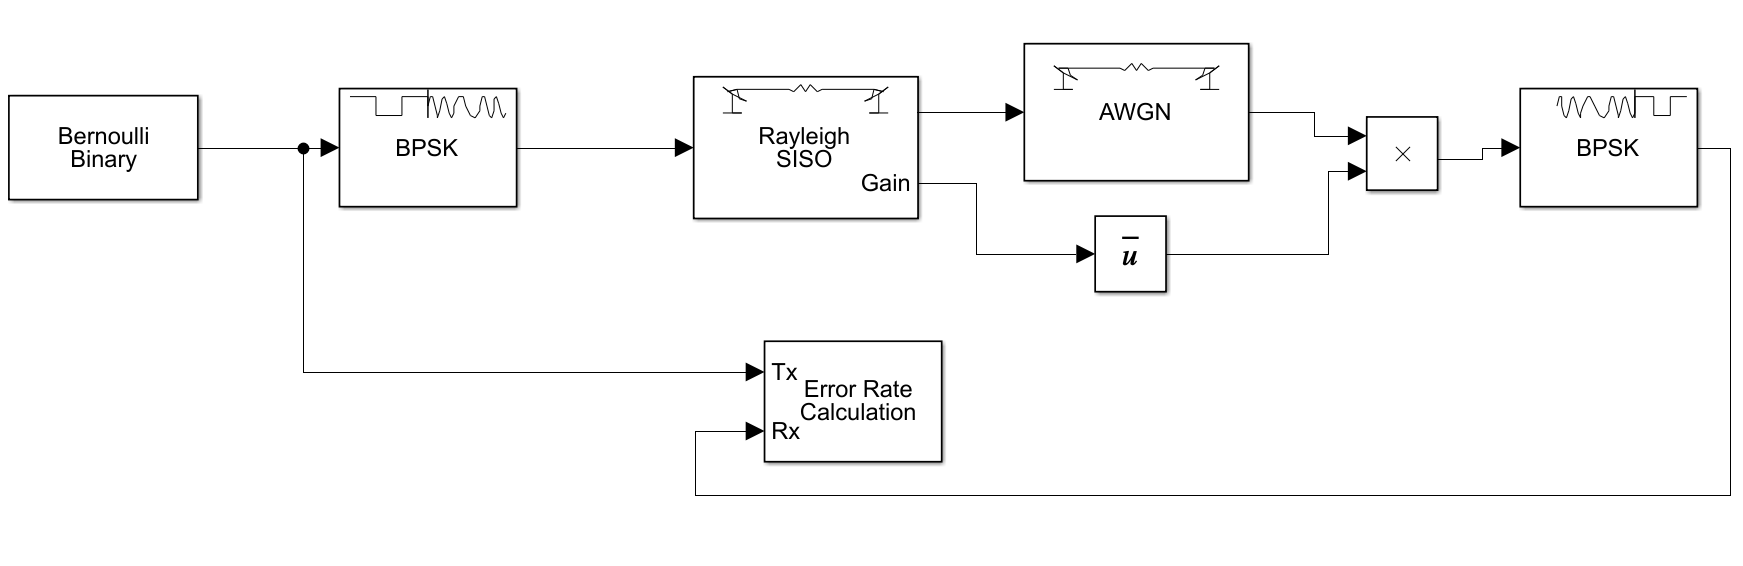
\includegraphics[width=\textwidth]{SimulinkModel-Task2_2}
   			\caption{Shows the model used for task 2.2}
   			\label{fig:2.2SimlinkModel}
   		\end{figure}
   	}
   	\subsection{Additive White Gaussian Noise}
   	{
   		This Module adds noise to the signal using the AWGN model, it allows us to replicate real world noise in our Simulink models.
   		\subsubsection{Parameters}
   		{
   			For this I needed to set the $\frac{E_b}{N_o}$ value to the Matlab workspace variable \lstinline|EbNo|. This allows the BERTool to change the signal to noise ratio when running the simulation. Also the symbol period must be correct as I am using a binary modulator this needs to match the sample time on the binary generator.
   		}
	}
	\subsection{BPSK Demodulator}
	{
		This converts the frequency data back into binary data 
	}
	\subsection{Error Rate Calculation}
	{
		This compares the output to the input and calculates the changes in the signal and outputs the error statistics. This gets outputted to a workspace variable called ErrorVec which is then accessible by the BERTool. I also had to change the maximum number of symbols from $10^6$ to $10^8$ as I was hitting the limit in my simulation.
	}
	\subsection{BER Tools}
	{
		I used Matlab's build in BerTool function to create some graphs for different fading models this would then allow me to use these as reference plots to compare to the results of my model this can be seen in \cref{fig:BerInital}.
		\begin{figure}
			\centering
			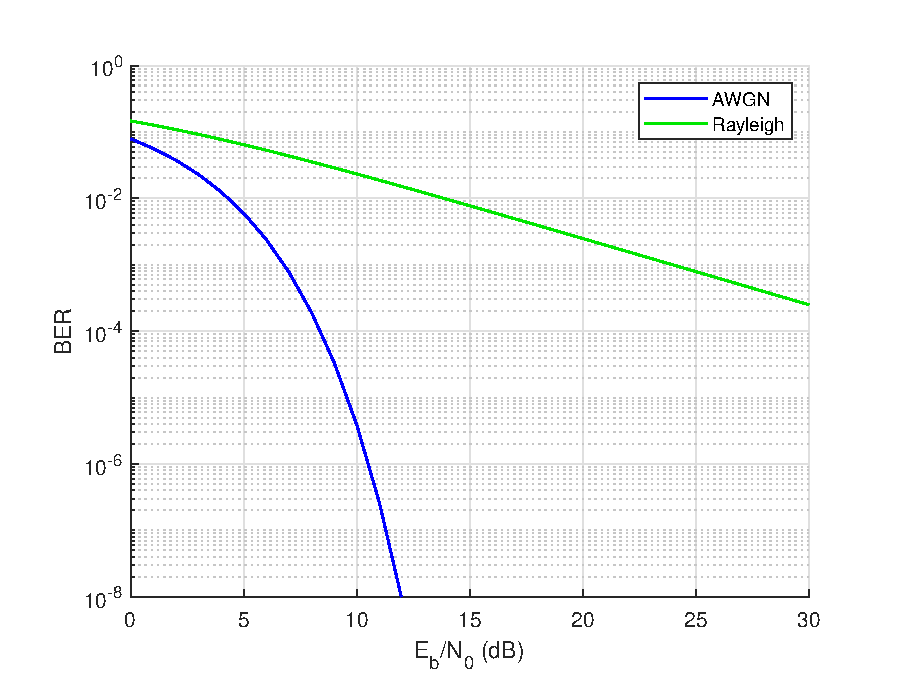
\includegraphics[width=\textwidth]{BERInital}
			\caption{Showing the theoretical AWGN and Rayleigh results}
			\label{fig:BerInital}
		\end{figure}
	}
	\subsection{First Model Analysis}
	{
		This is an example of a flat fading model as there is no Doppler value and a path delay of $10^{-6}$ also a data rate of 100 bits per second. As you can see from \cref{fig:BERModel1} the model is somewhere between a Rayleigh and AWGN model this is not surprising as it is a combination of both models as shown in \cref{fig:2.2SimlinkModel}. This model performs worse that then AWGN model however that is expected as that is the ideal curve. There is also clearly a factor of fast fading which is moving the curve above the Rayleigh curve.
   		\begin{figure}
			\centering
			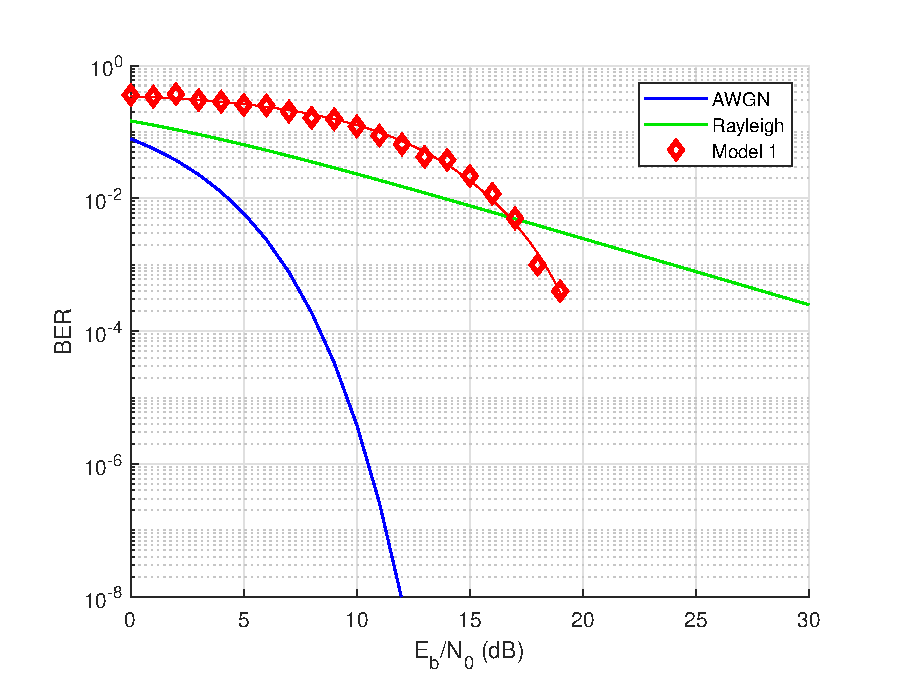
\includegraphics[width=\textwidth]{BERModel1}
			\caption{Shows the graph output for the first model along with two theoretical plots}
			\label{fig:BERModel1}
		\end{figure}
	}
	\subsection{Second Model Analysis}
	{
		For this section I set the Rayleigh path gain and delay to zero and changed the Doppler from 0 to 1Hz. \Cref{fig:BERModel2} shows the new plot as you can see it matches the Rayleigh relatively closely this is because when the values are low it appears the Rayleigh has more impact on the curve and as the $\frac{E_b}{N_o}$ gets larger the performance improves more like the AWGN curve.
   		\begin{figure}
			\centering
			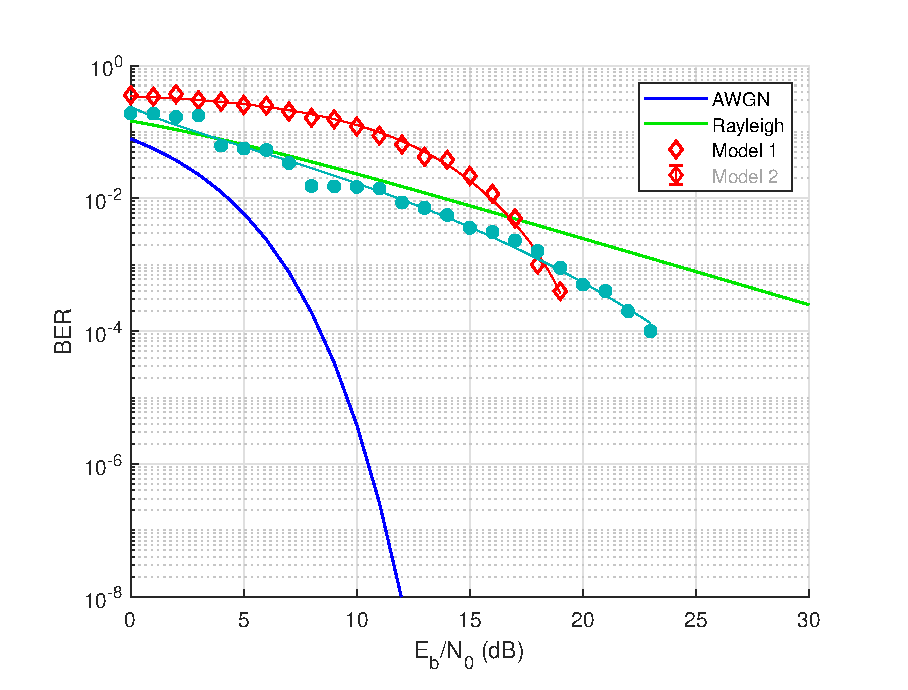
\includegraphics[width=\textwidth]{BERModel2}
			\caption{Shows the graph output for the second model along with the previous plots}
			\label{fig:BERModel2}
		\end{figure}
	}

}